\lab{Solitons}{Solitons}
\label{lab:solitons}
\labdependencies{NumericalIVP,SpectralMethod2}

\objective{Use a pseudospectral method to study solitons, the traveling wave solutions of the Korteweg-de Vries equation.}

The Korteweg-de Vries (KdV) equation is a partial differential equation given by
\[  \frac{\partial u }{\partial t} + u \frac{\partial u}{\partial x} + \frac{\partial^3 u}{\partial x^3} = 0.
\]
that describes shallow water waves.

The KdV equation possesses traveling wave solutions called \emph{solitons}.
These traveling waves have the form
\[ u(x,t) = 3s \sech^2\left(\frac{\sqrt{s}}{2}(x - st - a)\right),
\]
where $s$ is the speed of the wave.
Solitons were first studied by John Scott Russell in 1834, in the Union Canal in Scotland.
When a canal boat suddenly stopped, the water piled up in front of the boat continued moving down the canal in the shape of a pulse.

Note that there is a soliton solution for each wave speed $s$, and that the amplitude and speed of the soliton determine each other.
Solitons are nonlinearly stable (bumped waves return to their previous shape), and they maintain their energy as they travel.
Two interacting solitons will also both maintain their shapes after crossing paths.

\section*{Numerical solution}
Consider the KdV equation on $[-\pi,\pi]$, together with an appropriate initial condition:
\begin{align*}
	 &{ }u_t = -\frac{1}{2}\left(u^2 \right)_x - u_{xxx},\\
     &{ }u(x,0) = u_0(x).
\end{align*}
This form of the equation is slightly more convenient for the approach we will take.
We will suppose the initial condition is equal at the two endpoints; that is, \(u_0(-\pi)=u_0(\pi)\).
This will allow us to use the pseudospectral method to find a numerical approximation for the solution $u(x,t)$.

As a reminder, the pseudospectral method involves writing the solution at each point in time using a set of basis functions, complex exponentials being the most common, and using this representation to convert the PDE into an ODE.
Specifically, we can write any solution \(u(x,t)\) as
\[
u(x,t) = \sum_{k=-\infty}^\infty y_k(t)e^{ikx}.
\]
Recall that \(k\) is known as the wave number.
Note that all time-dependence of the solution is contained in the coefficients.
We can only compute this to some finite precision, so we will choose some \(n\) and truncate the series as
\[
u(x,t) = \sum_{k=-n}^n y_k(t)e^{ikx}.
\]
The objective is to obtain an ordinary differential equation for the coefficients \(y_k(t)\).
We now plug it into the PDE:
\begin{align*}
\frac{\partial}{\partial t}\sum_{k=-n}^n y_k(t)e^{ikx}
&=
-\frac{1}{2} \frac{\partial}{\partial x}\left(
\sum_{k=-n}^n y_k(t)e^{ikx}
\right)^2
-
\frac{\partial^3}{\partial x^3}\sum_{k=-n}^n y_k(t)e^{ikx}
\\
\sum_{k=-n}^n y_k'(t)e^{ikx}
&=
-\frac{1}{2} \frac{\partial}{\partial x}\left(
\sum_{k=-n}^n y_k(t)e^{ikx}
\right)^2
+
\sum_{k=-n}^n ik^3 y_k(t)e^{ikx}
\end{align*}
For this particular PDE, this leads to an apparent problem: the \(u^2\) term will be difficult and computationally costly to differentiate.
However, we can get around this difficulty using the fast Fourier transform.

Divide \([-\pi, \pi]\) into \(2n+1\) intervals of equal width \(\frac{2\pi}{2n+1}\), and let \(-\pi=x_{-n},x_{-n+1},\ldots,x_n,x_{n+1}=\pi\) be the \(2n+2\) evenly-spaced gridpoints.
For any function \(f\) on that interval with Fourier series \(f(x)=\sum_{k=-\infty}^\infty a_k e^{ikx}\), we can use the discrete Fourier transform on the values \(f(x_{-n}),\ldots,f(x_{n+1})\) at the gridpoints to quickly get the Fourier coefficients \(a_{-n},\ldots, a_n\).
The inverse Fourier transform can be used to get the function values at the grid points from the Fourier coefficients.
Both of these operations are very efficient, having complexity \(O(n\log n)\).
This sets up our strategy.

At each time \(t\), we can use the inverse Fourier transform to compute the values of \(u(x_m,t)\) for \(m=-n,\ldots,n+1\).
Then, we apply the Fourier transform to \(u^2\) to get its Fourier coefficients.
We will denote these as \(w_k\), so
\[
u^2(x,t)=\sum_{k=-n}^n w_k(t) e^{ikx}.
\]
Then,
\[
\frac{\partial}{\partial x}
u^2(x,t)=\sum_{k=-n}^n ik w_k(t) e^{ikx},
\]
so the KdV equation can be written as
\[
\sum_{k=-n}^n y_k'(t)e^{ikx}
=
\sum_{k=-n}^n \left(
-\frac{1}{2}ikw_k(t)
+
ik^3 y_k(t)
\right)e^{ikx}
\]
Equating terms in the Fourier series yields the ordinary system of differential equations
\[
y_k' = -\frac{1}{2}ikw_k + ik^3 y_k, \quad k=-n,\ldots, n.
\]
We can write this in a vectorized form as
\begin{equation}
\mathbf{y}' = -\frac{1}{2}i\mathbf{k}\odot\mathcal{F}(\mathcal{F}^{-1}(\mathbf{y})^2) + i\mathbf{k}^3 \odot\mathbf{y}
\label{lab:solitons:pseudospectral}
\end{equation}
where \(\mathcal{F}\) denotes the discrete Fourier transform.
In this equation, all of the multiplication and exponentiation is componentwise.

To obtain the initial condition for the \(y_k\), we can simply use the discrete Fourier transform again:
\[
\mathbf{y}(0) = \mathcal{F}(u_0(x_{-n}),\ldots,u_0(x_{n+1}))
\]

To compute the fast Fourier and inverse fast Fourier transforms numerically, we will use the \li{scipy.fft} module, which has functions \li{fft} for the fast Fourier transform and \li{ifft} for the inverse fast Fourier transform.
These functions use an order for the coefficients that is slightly nonintuitive: the coefficients for \(k\geq 0\) are all listed first, followed by the coefficients for \(k<0\).
The vector of wavenumbers can be created as follows:
\begin{lstlisting}
k = np.concatenate([
        np.arange(0, n+1),
        np.arange(-n-1, 0)
])
\end{lstlisting}
We are now prepared to numerically solve the KdV equation.

\begin{problem}
Write a function that accepts the time value \(t\) (which won't be used here, but will be useful later) the vector \(\mathbf{y}=(y_0,y_1,\ldots,y_n,y_{-n-1},\ldots,y_{-1})\) and the vector \(\mathbf{k}\) of wavenumbers and returns \(\mathbf{y}'\) as given in (\ref{lab:solitons:pseudospectral}).
\end{problem}

\noindent To numerically solve this ODE, we'll use \li{solve_ivp}.
For this lab we want to specify a fixed time step size to use with the RK4 algorithm, but \li{scipy}'s implementation uses an adaptive method to control the time step.
So we've defined an RK4 implementation that can be passed into \li{solve_ivp} with the \li{method} argument, and we provide the time step \li{dt} through the call to \li{solve_ivp}.
\begin{lstlisting}
from scipy.integrate import solve_ivp, OdeSolver
from scipy.integrate._ivp.common import warn_extraneous

class RK4(OdeSolver):
    def __init__(self, fun, t0, y0, t_bound, dt, vectorized, **extraneous):
        super().__init__(fun, t0, y0, t_bound, vectorized, support_complex=True)

        self.dt = dt

        # t-linspace
        self.tls = np.arange(0, t_bound + dt, dt)

        self.idx = iter(range(1, len(self.tls)))

        warn_extraneous(extraneous)

    def _step_impl(self):
        self.y_old = self.y

        i = next(self.idx)
        t = self.tls[i]
        y = self.y
        f = self.fun
        dt = self.dt

        # RK4 algorithm
        K1 = f(t, y)
        K2 = f(t + dt / 2, y + dt * K1 / 2)
        K3 = f(t + dt / 2, y + dt * K2 / 2)
        K4 = f(t + dt, y + dt * K3)
        y_new = y + (dt / 6) * (K1 + 2 * K2 + 2 * K3 + K4)

        self.t = t
        self.y = y_new
        return True, None

    def _dense_output_impl(self):
        return lambda xs: np.interp(
            xs, (self.t_old, self.t), (self.y_old, self.y)
        )

# `args` is passed to the ODE function you defined in Problem 1.
# `dt` is passed to `RK4`.
sol = solve_ivp(..., args=(k,), method=RK4, dt=dt)
\end{lstlisting}

Once we have solved for the coefficients \(\mathbf{y}(t)\), we need to convert them back into function values \(u(x,t)\) in order to visualize the solution.
This is accomplished by using the \li{ifft} function on the coefficient values at each time step.
However, this function is designed to work with complex numbers, and returns a complex-valued array.
Due to numerical error, even though our ODE solution is real-valued, there may be small imaginary components to the result; use \li{np.real} on the result to discard these.

\begin{problem}
Write a function that accepts an initial condition \(u_0\), a final time \li{T}, the timestep \li{dt}, an integer \(n\) for the number of coefficients to use, and another integer \li{skip}.
Numerically solve for the coefficients \(\mathbf{y}(t)\) of a solution to the KdV equation.

Next, convert the Fourier coefficients back into function values at the gridpoints using the inverse Fourier transform.
However, only do this for every \li{skip}-th timestep; we will be using far more timesteps than we want to plot.
Return the gridpoints, the timesteps, and the solution \(u(x,t)\).
\end{problem}

\noindent
Once we have the function values, we can plot them as a surface as follows:
% could always change it to an animation :)
\begin{lstlisting}
fig = plt.figure()
ax = fig.add_subplot(1,1,1, projection="3d")

T, X = np.meshgrid(t, x, indexing="ij")
ax.plot_surface(T, X, u, cmap="coolwarm", rstride=1, cstride=1)
\end{lstlisting}
%This creates a 3-d plot, so the subplot this is done in must be created with \li{projection="3d"}.

\begin{problem}
Numerically solve the KdV equation on $[-\pi,\pi]$ with initial conditions
\[
u(x,t=0) = 3s\sech^2\left(\frac{\sqrt{s}}{2}(x+a)\right),
\]
where $s = 25^2,$ $a = 2$. Solve on the time domain $[0,0.0075]$, and use \(n=127\).
Compare with Figure \ref{fig:solitons:single}; to get a similar viewpoint, use the following:
\begin{lstlisting}
ax.view_init(elev=45, azim=-45)
ax.set_zlim(0, 4000)
ax.invert_xaxis()
\end{lstlisting} %TODO update the figure
How small of a timestep did you need to use for the numerical integration to be stable?
(Hint: it's smaller than $10^{-5}$.)
If your solution becomes full of NaN values, you are most likely using too large of a timestep.
\label{problem:solitons:single}

\noindent
Hint: \li{numpy} does not have a \li{sech} function; use \li{1/cosh(x)} to compute it instead.
\end{problem}

\begin{figure}[H]
\centering
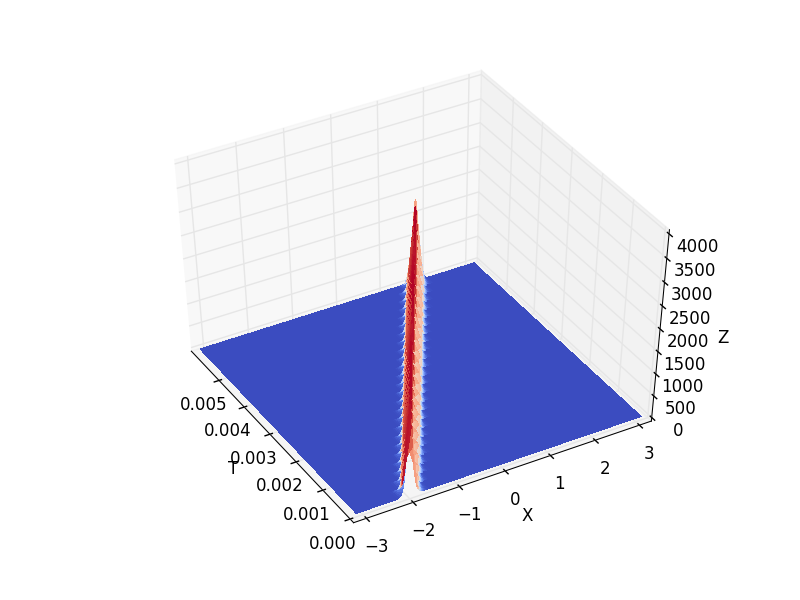
\includegraphics[width=\textwidth]{figures/soliton.pdf}
\caption{The solution to Problem \ref{problem:solitons:single}.}
\label{fig:solitons:single}
\end{figure}

\begin{problem}
Numerically solve the KdV equation on $[-\pi,\pi]$.
This time we define the initial condition
to be the superposition of two solitons:
\[
u(x,t=0) = 3s_1\sech^2\left(\frac{\sqrt{s_1}}{2}(x+a_1)\right) + 3s_2\sech^2\left(\frac{\sqrt{s_2}}{2}(x+a_2)\right),
\]
where $s_1 = 25^2,$ $a_1 = 2$, and $s_2 = 16^2,$ $a_2 = 1$.\footnote{This problem is from \textit{Spectral Methods in MATLAB}, by Trefethen.}
Solve on the time domain $[0,0.0075]$.
The solution is shown in Figure \ref{fig:solitons:interacting}.
\label{problem:solitons:interacting}
\end{problem}

\begin{figure}[H]
\centering
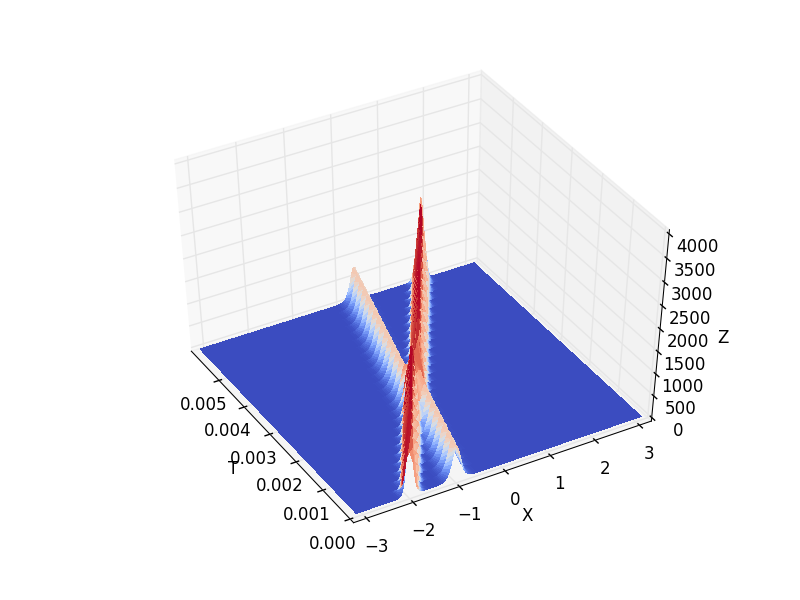
\includegraphics[width=\textwidth]{figures/interacting_solitons.pdf}
\caption{The solution to Problem \ref{problem:solitons:interacting}.}
\label{fig:solitons:interacting}
\end{figure}

\begin{problem}
Consider again equation \eqref{lab:solitons:pseudospectral}.
The linear term in this equation is $i\mathbf{k}^3\mathbf{y}$.
This term contributes much of the exponential growth in the ODE, and contributes to how short the time step must be to ensure numerical stability.
Make the substitution $z_k(t) = e^{-ik^3t}y_k(t)$ and find a similar ODE for $\mathbf{z}$.
This essentially allows the exponential growth to be scaled out (it's solved for analytically, replacing it with rotation in the complex plane).
Use the resulting equation to solve the previous problem.
How much larger of a timestep can you use while this method remains stable?
\end{problem}
